\sectionframe{Data sources}
\subsection{Excel spreadsheets}
\begin{frame}
 \frametitle{Building a \texttt{SheetConnection}}
 The object data type \texttt{SheetConnection} connects to an Excel spreadsheet (MS Windows only)
 \begin{block}{Construction of a \texttt{SheetConnection}}
  \ttfamily
  SheetConnection \textsf{\slshape name}("\textsf{\slshape path to spreadsheet}");
 \end{block}
 \begin{block}{Possible data types for reading and writing}
  \begin{itemize}
   \item zero-dimensional data types, i.e. single variables. Reading data from one cell.
   \item one-dimensional data types, i.e. sets and single arrays. Reading data from a row or column.
   \item two-dimensional data types, i.e. double arrays. Reading data from a cell matrix.
  \end{itemize}
 \end{block}
\end{frame}

\begin{frame}
 \frametitle{Reading and writing with absolute cell adressing}
 \begin{block}{Reading with absolute cell adressing}
  \ttfamily
  \textsf{\slshape variable name} from SheetRead(\textsf{\slshape SheetConnection name}, "\textsf{\slshape table name}!\textsf{\slshape starting cells}:\textsf{\slshape ending cell}")
 \end{block}
 \begin{block}{Writing with absolute cell adressing}
  \ttfamily
  \textsf{\slshape variable name} to SheetWrite(\textsf{\slshape SheetConnection name}, "\textsf{\slshape table name}!\textsf{\slshape starting cell}:\textsf{\slshape ending cell}")
 \end{block}
\end{frame}

\begin{frame}[fragile]
 \frametitle{In example ``Vindoo Support''}
 \begin{block}{Excel spreadsheet for example ``Vindo Support''}
  \centering
  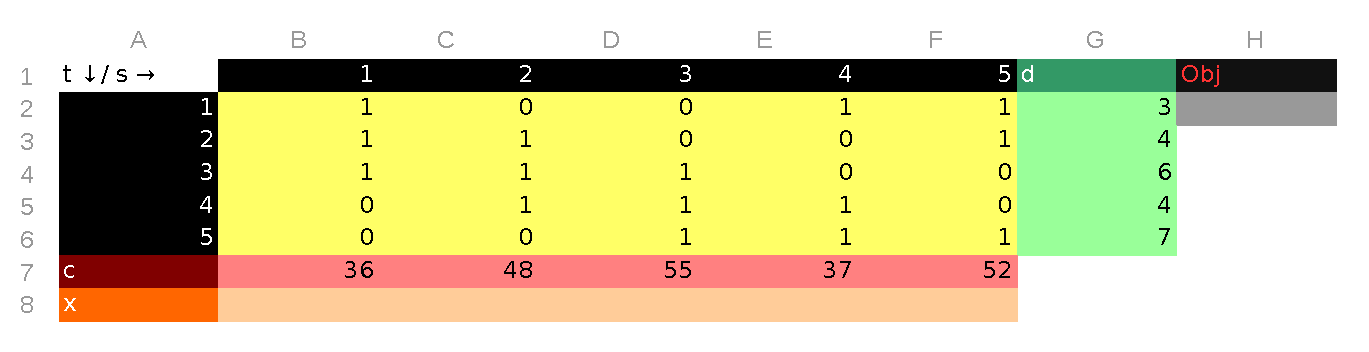
\includegraphics[width=.9\linewidth]{Bilder/CyclicStaffingData}
 \end{block}
 \begin{block}{Excerpt from the data file}
\begin{lstlisting}[language=opldata,numbers=none,basicstyle=\ttfamily\scriptsize]
// SheetConnection
SheetConnection sheet("CyclicStaffingProblem.xls");
\end{lstlisting}\vspace{-2\baselineskip}
\begin{lstlisting}[language=opldata,numbers=none,basicstyle=\ttfamily\scriptsize]
// index sets
T from SheetRead(sheet, "Data!B1:F1");
\end{lstlisting}\vspace{-2\baselineskip}
\begin{lstlisting}[language=opldata,numbers=none,basicstyle=\ttfamily\scriptsize]
//parameters
d from SheetRead(sheet, "Data!G2:G6");
\end{lstlisting}\vspace{-2\baselineskip}
\begin{lstlisting}[language=opldata,numbers=none,basicstyle=\ttfamily\scriptsize]
//decision variables
x to SheetWrite(sheet, "Data!B8:F8");
\end{lstlisting}
 \end{block}
\end{frame}

\begin{frame}
 \frametitle{Reading and writing with named ranges}
 In MS Excel it is possible to name cell ranges.
 \begin{block}{Reading with named ranges}
  \ttfamily
  \textsf{\slshape variable name} from SheetRead(\textsf{\slshape SheetConnection name}, "\textsf{\slshape range name}")
 \end{block}
 \begin{block}{Writing with named ranges}
  \ttfamily
  \textsf{\slshape variable name} to SheetWrite(\textsf{\slshape SheetConnection name}, "\textsf{\slshape range name}")
 \end{block}
\end{frame}

\begin{frame}[fragile]
 \frametitle{In example ``Vindoo Support''}
 \begin{block}{Excel spreadsheet for example ``Vindo Support''}
  \begin{center}
   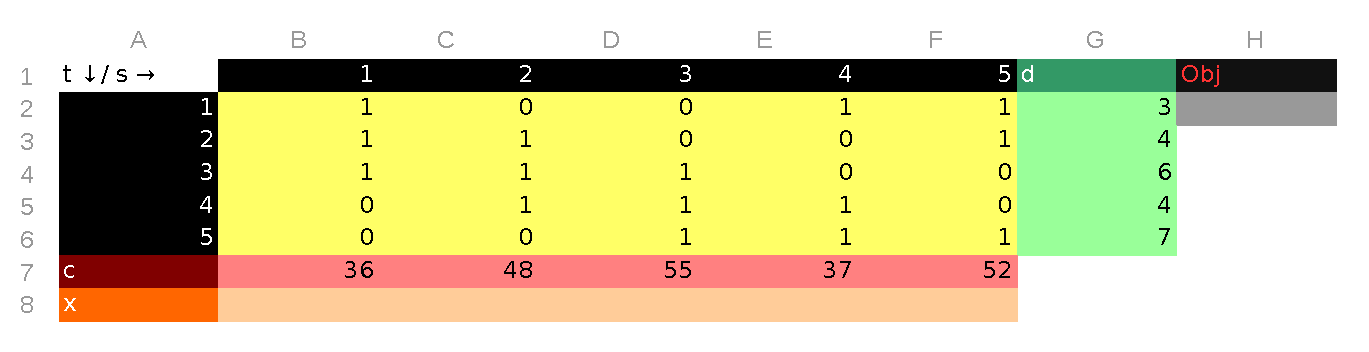
\includegraphics[width=.9\linewidth]{Bilder/CyclicStaffingData}
  \end{center}\vspace{-1\baselineskip}
  The yellow range is named ``\texttt{ParamA}''
 \end{block}
 \begin{block}{Excerpt from the data file}
\begin{lstlisting}[language=opldata,numbers=none,basicstyle=\ttfamily\scriptsize]
// SheetConnection
SheetConnection sheet("CyclicStaffingProblem.xls");
\end{lstlisting}\vspace{-2\baselineskip}
\begin{lstlisting}[language=opldata,numbers=none,basicstyle=\ttfamily\scriptsize]
//parameters
a from SheetRead(sheet, "ParamA");
\end{lstlisting}
 \end{block}
\end{frame}

\subsection{Data bases}
\begin{frame}
 \frametitle{Building a \texttt{DBConnection}}
 The object data type \texttt{DBConnection} connects to a data base.
 \begin{block}{Construction of a \texttt{DBConnection}}
  \ttfamily
  DBConnection \textsf{\slshape name}("\textsf{\slshape interface}", "\textsf{\slshape connection string}");
 \end{block}
 \begin{block}{Supported data base interfaces}
  \begin{itemize}
   \item DB2
   \item Oracle (Version 10 und 11)
   \item OLE DB (MS SQL Server)
   \item ODBC (u.a. für MS Access)
  \end{itemize}
 \end{block}
\end{frame}

\begin{frame}
 \frametitle{example data base: \texttt{CyclicStaffingProblem}}
 \begin{table}[htbp]\tiny
 \begin{tabularx}{\linewidth}{XX}
  \begin{minipage}{\linewidth}
   \begin{subtable}[b]{\linewidth}
     \centering
     \begin{tabular}{ccc}
      \toprule
      \ttfamily s 
\includegraphics[width=1em]{Bilder/Key} & \ttfamily t 
\includegraphics[width=1em]{Bilder/Key} & \ttfamily a \\
      \midrule
      \arrayrulecolor{gray!30}
      1 & 1 & 1 \\
      1 & 2 & 1 \\
      1 & 3 & 1 \\
      1 & 4 & 0 \\
      1 & 5 & 0 \\
      \midrule
      2 & 1 & 0 \\
      2 & 2 & 1 \\
      2 & 3 & 1 \\
      2 & 4 & 1 \\
      2 & 5 & 0 \\
      \midrule
      3 & 1 & 0 \\
      3 & 2 & 0 \\
      3 & 3 & 1 \\
      3 & 4 & 1 \\
      3 & 5 & 1 \\
      \midrule
      4 & 1 & 1 \\
      4 & 2 & 0 \\
      4 & 3 & 0 \\
      4 & 4 & 1 \\
      4 & 5 & 1 \\
      \midrule
      5 & 1 & 1 \\
      5 & 2 & 1 \\
      5 & 3 & 0 \\
      5 & 4 & 0 \\
      5 & 5 & 1 \\
      \arrayrulecolor{black}
      \bottomrule
     \end{tabular}
    \caption{table \texttt{A}}
    \end{subtable}
  \end{minipage}
  &
  \begin{minipage}{\linewidth}
    \begin{subtable}[b]{\linewidth}
     \centering
     \begin{tabular}{cc}
      \toprule
      \ttfamily ind 
\includegraphics[width=1em]{Bilder/Key} & \ttfamily d \\
      \midrule
      1 & 2 \\
      2 & 4 \\
      3 & 6 \\
      4 & 4 \\
      5 & 7 \\
      \bottomrule
     \end{tabular}
    \caption{table \texttt{T}}
    \end{subtable}
    \bigskip\bigskip
    
    \begin{subtable}[b]{\linewidth}
     \centering
     \begin{tabular}{ccc}
      \toprule
      \ttfamily ind 
\includegraphics[width=1em]{Bilder/Key} & \ttfamily c & \ttfamily x \\
      \midrule
      1 & 36 \\
      2 & 48 \\
      3 & 55 \\
      4 & 37 \\
      5 & 52 \\
      \bottomrule
     \end{tabular}
    \caption{table \texttt{S}}
    \end{subtable}
  \end{minipage}
 \end{tabularx}
\end{table}
\end{frame}

\begin{frame}[fragile]
 \frametitle{Reading array data}
 The example data base \texttt{CyclicStaffingProblem} shall be connected via an ODBC interface. The user ``\texttt{user}'' with the password ``\texttt{password}'' has the necessary rights to access the data base.
 \begin{block}{Excerpt from the data file}
\begin{lstlisting}[language=opldata,numbers=none,basicstyle=\ttfamily\scriptsize]
// DBConnection
DBConnection 
  db("odbc", "CyclicStaffingProblem/user/password");
\end{lstlisting}\vspace{-2\baselineskip}
\begin{lstlisting}[language=opldata,numbers=none,basicstyle=\ttfamily\scriptsize]
// index sets
T from DBRead (db, "SELECT ind from T");
\end{lstlisting}\vspace{-2\baselineskip}
\begin{lstlisting}[language=opldata,numbers=none,basicstyle=\ttfamily\scriptsize]
// parameters
c from DBRead(db, "SELECT ind,c from S");
a from DBRead(db, "SELECT t,s,a from A");
\end{lstlisting}
 \end{block}
\end{frame}

\begin{frame}[fragile]
 \frametitle{Reading and writing of tuple data}
 \begin{block}{Excerpt from the model file}
\begin{lstlisting}[language=opl,numbers=none,basicstyle=\ttfamily\scriptsize]
//Tuple
tuple shift{
  int ind;
  float c;
}
tuple result{<
  int x;
  int ind;
}  
\end{lstlisting}\vspace{-2\baselineskip}
\begin{lstlisting}[language=opl,numbers=none,basicstyle=\ttfamily\scriptsize]
//Postprocessing
{result} r = {<x[s],s.ind>|s in S};
\end{lstlisting}
 \end{block}\vspace{-2\baselineskip}
 \begin{block}{Excerpt from the data file}
\begin{lstlisting}[language=opldata,numbers=none,basicstyle=\ttfamily\scriptsize]
//index sets
S from DBRead(db, "SELECT ind,c from S");
\end{lstlisting}\vspace{-2\baselineskip}
\begin{lstlisting}[language=opldata,numbers=none,basicstyle=\ttfamily\scriptsize]
//decision variables
r to DBUpdate(db, "UPDATE S SET x=? WHERE ind=?");
\end{lstlisting}
 \end{block}
\end{frame}

